\documentclass[]{article}
\usepackage{atlasphysics}
% Nice maths macros
\usepackage{amsmath}
% Units
\usepackage{siunitx}
% Figures and floats
\usepackage{graphicx,subfigure,float}

% Graphics folider
\graphicspath{{figures/}}

% Scientific notation
% http://www.tapdancinggoats.com/easy-scientific-notation-in-latex.htm
\providecommand{\e}[1]{\ensuremath{\times 10^{#1}}}
% Differential Operator
\renewcommand{\d}[1]{\ensuremath{\,\operatorname{d}\!{#1}}}
% Absolute value
\renewcommand{\mod}[1]{\ensuremath{\lvert {#1} \rvert}}
% Airys functions Ai(x) and Bi(x)
\newcommand{\Ai}[1]{\ensuremath{\operatorname{Ai}({#1})}}
\newcommand{\Bi}[1]{\ensuremath{\operatorname{Bi}({#1})}}

\begin{document}

\title{Masses of S-State Mesons via the Roots of Airy's Function $\Ai{x}$}
\author{Alex Pearce}
\date{\today}
\maketitle


\begin{abstract}
\end{abstract}

\section{Introduction}\label{sec:intro}


\section{Figures}\label{sec:figures}

\begin{figure}[H]
	\hspace*{-0.15\textwidth}
	\centering
	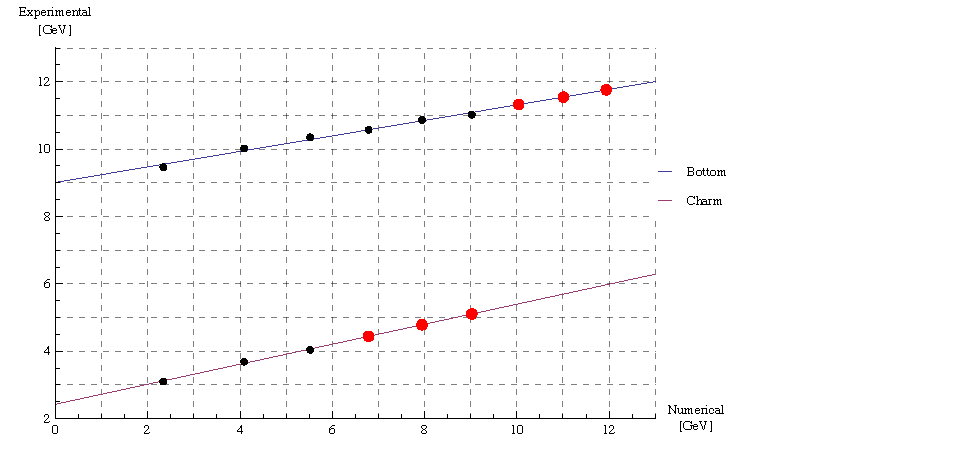
\includegraphics[scale=1.3]{experimental-numerical}
	\caption{TODO: Caption here}
	\label{fig:data}
\end{figure}


\begin{thebibliography}{9}
	\bibitem{ref:gjdaniell}
  G. J. Daniell,
  \emph{PHYS6017 Course Notes},
  University of Southampton, Southampton, UK,
  2011.
  
	\bibitem{ref:agil}
  A. Gil, J. Segura and N. M. Temme,
  \emph{Numerical Methods for Special Functions},
  Society for Industrial and Applied Mathematics, Philadelphia PA, USA,
  $1$st Edition,
  2007.
  
  \bibitem{ref:nr}
  W. H. Press et al.,
  \emph{Numerical Recipes: The Art of Scientific Computing},
  Cambridge University Press, Cambridge, UK,
  $3$rd Edition,
  2007
  
\end{thebibliography}

\end{document}